% figures/story_captions.tex
% Generated by src/analysis/make_story_figures.py on 2026-09-11.
% Every number below was computed by that script from the same arrays it
% plotted; do not edit them by hand. CR data SHA-8 710f4a24
% (L_grid sha256 2d92b58e1693107d...).
%
% Usage:  % figures/story_captions.tex
% Generated by src/analysis/make_story_figures.py on 2026-09-11.
% Every number below was computed by that script from the same arrays it
% plotted; do not edit them by hand. CR data SHA-8 710f4a24
% (L_grid sha256 2d92b58e1693107d...).
%
% Usage:  % figures/story_captions.tex
% Generated by src/analysis/make_story_figures.py on 2026-09-11.
% Every number below was computed by that script from the same arrays it
% plotted; do not edit them by hand. CR data SHA-8 710f4a24
% (L_grid sha256 2d92b58e1693107d...).
%
% Usage:  % figures/story_captions.tex
% Generated by src/analysis/make_story_figures.py on 2026-09-11.
% Every number below was computed by that script from the same arrays it
% plotted; do not edit them by hand. CR data SHA-8 710f4a24
% (L_grid sha256 2d92b58e1693107d...).
%
% Usage:  \input{figures/story_captions.tex}  in the preamble, then
%   \begin{figure}[t]\centering
%     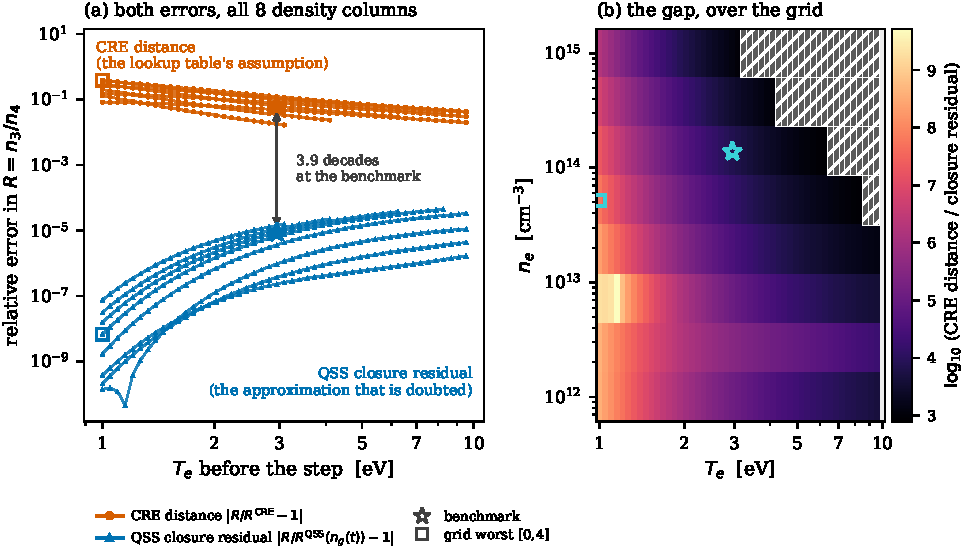
\includegraphics{figures/fig5_5_reversal.pdf}
%     \caption{\CapFigReversal}\label{fig:reversal}
%   \end{figure}

\newcommand{\CapFigReversal}{%
  \textbf{The reversal: the approximation that is doubted holds, the
  assumption that is not examined fails.}
  Two errors in the same observable, the shell ratio $R = n_3/n_4$, measured
  along the same trajectory after a $+4.81\%$ step in $T_e$ at fixed $n_e$,
  and reported as the maximum over the timescale-separated plateau window
  $30\tau_{\rm relax} < t < \tau_{\rm slow}/30$.
  The \emph{quasi-steady-state closure residual} is
  $|R(t)/R^{\rm QSS}(n_g(t)) - 1|$, where $R^{\rm QSS}$ is rebuilt at each
  instant from the excited-state block alone,
  $n_E = -L_{EE}^{-1}(L_{Eg}n_g + S_E)$, evaluated at the
  \emph{instantaneous} ground density rather than at any tabulated value.
  The \emph{CRE distance} is $|R(t)/R^{\rm CRE} - 1|$, the distance to the
  equilibrium-ionisation-balance state $n = -L^{-1}S$ that a two-parameter
  $(T_e, n_e)$ lookup table returns.
  (a) Both, for all 392 analysed cells across the 8 density
  columns. The closure residual runs from $4.6\times10^{-11}$ to $4.4\times10^{-5}$, so the
  closure everyone worries about is never worse than one part in
  $2.2\times10^{4}$ anywhere on the analysed grid: it is $8.66\times10^{-6}$ at the
  benchmark ($T_e = 2.947$~eV, $n_e = 1.4\times10^{14}$~cm$^{-3}$), one part in
  $1.2\times10^{5}$, and $6.73\times10^{-9}$ at the coldest point
  $[0,4]$, one part in $1.5\times10^{8}$.
  The CRE distance over the same cells runs from 1.66\% to 38.7\%:
  6.34\% at the benchmark and 38.7\% at the coldest point.
  The assumption nobody examines therefore fails at the tens-of-percent
  level exactly where the closure everybody examines is exact to within
  one part in $10^{5}$ or better.
  (b) The ratio of the two over the grid. The gap is 2.9 to 9.7
  decades wide, 3.9 decades at the benchmark and 7.8 decades at the
  coldest point; it is not a single number and should not be quoted as one.
  Hatched cells (54 of 392) have no timescale-separated plateau
  window, $M \leq 900$, an imposed cut rather than a measured floor.
  Trajectories are eigen-propagations of the full 43-state operator,
  sampled at 24 points across each window and checked against
  \texttt{scipy.linalg.expm} at the window midpoint of every cell, worst
  disagreement $3\times10^{-9}$.
  Values below $2$~eV are optically thin upper estimates: Lyman trapping is
  not switched on here.}

\newcommand{\CapFigTrajectory}{%
  \textbf{What the plateau looks like: the excited states keep up, the
  reservoir does not.}
  The shell ratio $R(t) = n_3/n_4$ after a step in $T_e$ at fixed $n_e$,
  on a logarithmic time axis long enough to hold both timescales.
  Three phases are visible. $R$ rises on $\tau_{\rm relax}$ as the excited
  manifold re-equilibrates against a ground state that has not yet moved; it
  sits at the partial-equilibrium value $R^{\rm PE}$; then it decays on
  $\tau_{\rm slow}$ as the ground state, and with it the ionisation balance,
  finally responds. The excited states are fast enough to track the new
  temperature within nanoseconds. The reservoir that feeds them is not.
  (a) The benchmark, $T_e = 2.947 \rightarrow 3.09$~eV at
  $n_e = 1.4\times10^{14}$~cm$^{-3}$: $R$ moves from $0.7778$ through
  $0.8201$ to $0.7711$, a plateau error of 6.36\%, with
  $\tau_{\rm relax} = 2.24\times10^{-9}$~s and $\tau_{\rm slow} = 1.85\times10^{-5}$~s
  ($M = 8243$).
  (b) The coldest grid point, $T_e = 1.00 \rightarrow 1.05$~eV at
  $n_e = 5.2\times10^{13}$~cm$^{-3}$: $1.2391$ through $1.6712$ to $1.2050$,
  38.7\%, with $\tau_{\rm relax} = 6.24\times10^{-9}$~s and
  $\tau_{\rm slow} = 0.233$~s ($M = 3.74\times10^{7}$), five orders of magnitude of
  separation between the two clocks.
  Every timescale quoted belongs to the \emph{post-step} operator, the one
  that governs the relaxation; the same grid point read from its unstepped
  operator gives a different $M$, and the two must not be interchanged.
  $R^{\rm PE}$ is computed independently by a single linear solve against
  that operator and agrees with the two-channel construction used elsewhere
  in this chapter to $2\times10^{-16}$. The plateau is flat to 0.17\%
  peak to peak in (a). Curves are eigen-propagations of the full
  43-state operator, cross-checked against \texttt{scipy.linalg.expm}
  inside the plateau window, worst disagreement $1\times10^{-7}$.}

\newcommand{\CapFigStructuralMaps}{%
  \textbf{The two structural coefficients, and the invariant they multiply
  to.}
  The plateau error obeys
  $\varepsilon = |\exp(\bar{S} G \,\mathrm{d}\ln T_e) - 1|$ exactly, which
  splits it into a part belonging to the observable and a part belonging to
  the plasma.
  (a) $|\bar{S}| = |f_3 - f_4|$, the sensitivity of the $n=3/n=4$ ratio to
  the ground-state reservoir, where $f_n$ is the ground-fed fraction of shell
  $n$.
  (b) $|G| = |\mathrm{d}\ln u / \mathrm{d}\ln T_e|$, the reservoir gain,
  measuring how far the ground population moves for a given change in
  temperature.
  (c) Their product $|\bar{S}G|$, which is the small-step limit of
  $\varepsilon/|\mathrm{d}\ln T_e|$ and is the coefficient this chapter reports
  in place of a percentage that depends on the step chosen. It is written as a
  limiting ratio and not as $\mathrm{d}\varepsilon/\mathrm{d}\ln T_e$ because
  $\varepsilon = |\mathrm{e}^z-1|$ has a corner at $z=0$, where the two-sided
  derivative does not exist. $G$ itself is a secant over the step taken, not a
  local derivative, so it carries a weak and systematic step dependence.
  All three are heating, one grid index in $T_e$
  ($\mathrm{d}\ln T_e = 0.0470$), over all 392 cells.
  Ranges quoted with their scope, because the scope changes them: over the
  338 cells drawn here that pass the plateau-window test,
  $|\bar{S}|$ runs 0.065 to 0.482 and $|G|$ runs 2.64 to 14.52, giving
  a product of 0.36 to 6.96; over all 2288 rows of the source table,
  which include cooling and larger steps, $|\bar{S}|$ runs 0.0355 to
  0.4963 while $|G|$ is unchanged at 2.64 to 14.52.
  At the benchmark $|\bar{S}| = 0.229$, $|G| = 5.74$ and the product is
  1.31.
  $G$ is what makes this reframing worth anything: across step sizes of one,
  two and four grid indices at the 736 points carrying all three, $|G|$
  varies by at most 6.74\% (median 1.0555) while $\varepsilon$ over
  the same points varies by up to a factor 8.44.
  Hatched cells (54 of 392) fail the plateau-window test
  $M > 900$; their values are drawn rather than deleted, since $\bar{S}$
  and $G$ are properties of the operator and remain defined there even where
  a plateau does not.}

\newcommand{\CapFigScope}{%
  \textbf{Two independent constraints put the same floor under the
  quantitative scope.}
  Neither boundary was chosen; both were measured, and they come from
  unrelated physics.
  \emph{Quasi-neutrality.} Imposing nuclei conservation across one grid step
  in $T_e$, the electron density must change by
  $|\Delta n_e / n_e| = |\Delta n_g| / n_{\rm ion}$, taken from the two
  CR-equilibrium solves either side of the step. This zero-dimensional model
  holds $n_e$ fixed, so wherever that requirement is large the model is
  contradicting itself. Of the 392 one-step operators on the grid,
  68 require more than $10\%$ and 36 require more than $100\%$. At
  $T_e = 1$~eV the requirement is between 10.1 and 20.0, that
  is, ten to twenty times the electron density itself. At $T_e \geq 2$~eV it
  never exceeds $0.0054$. The $10\%$ contour sits at
  $T_e = 1.41$ to 1.50~eV and is almost independent of density.
  \emph{Optical depth.} The Lyman-$\alpha$ line-centre optical depth over the
  half slab, $\tau_0 = n(1s)\,\sigma_0\,D/2$, with $\sigma_0$ evaluated at
  $T_{\rm at} = T_e$ from the Doppler width $\sqrt{2kT/m}$, giving
  $\sigma_0 = 5.474\times10^{-14}$~cm$^{2}$ at $1$~eV. The optically thin matrix used
  throughout this thesis is only defensible where $\tau_0 < 1$. That contour
  runs from $T_e = 1.13$ to 1.98~eV at the slab thickness
  $D = 5$~cm, and across the 3 thicknesses in the trapping sweep it
  spans 1.01 to 2.36~eV.
  (a) Both boundaries on the $(T_e, n_e)$ plane, over a map of the
  quasi-neutrality requirement.
  (b) Each constraint divided by its own limit, so that a value above one
  means the constraint is violated and the two can share a single axis.
  Both boundaries fall between 1.01 and 2.36~eV. Two independent
  pieces of physics, particle conservation and radiation transport, place the
  floor in the same narrow band, and $T_e \geq 2$~eV clears both everywhere
  except 2 of the 3 times eight optical-depth crossings, which sit
  at the largest slab thickness $D = 20$~cm and the two highest density
  columns. The $T_e \geq 2$~eV restriction is therefore a measured boundary,
  not a hedge.}

\newcommand{\CapFigDiagnosticChain}{%
  \textbf{Where the hidden assumption enters divertor spectroscopy.}
  The inference runs left to right. A spectrometer records the Balmer
  emission; the ratio of two line intensities, here
  $I_{{\rm H}\alpha}/I_{{\rm H}\beta}$ at $656.1$ and $486.0$~nm, reduces
  the spectrum to a single number per line of sight; that number is looked up
  in a table of the ratio computed as a function of $(T_e, n_e)$; and the
  pair that reproduces it is reported as the plasma conditions.
  The step that is rarely stated is the third. The table is built from the
  CR-equilibrium populations, so it assumes the ionisation balance has
  already settled, $n_g/n_{\rm ion} = u^{\rm CRE}(T_e, n_e)$. A plasma still
  in transit after a change in temperature does not satisfy that, and the
  inversion then returns a temperature and a density that no plasma had.
  This thesis is about the size of that error and about which of the
  approximations in the chain is actually responsible for it.
  This is a schematic. No measured or computed quantity is plotted; the two
  wavelengths are the only numbers on it, and they follow from the
  ionisation energies in the model's own state index. The drawn line heights
  are arbitrary and carry no information about the real intensity ratio.}

\newcommand{\CapFigStateSpace}{%
  \textbf{The 43-state space and the five processes the rate matrix
  contains.}
  Left: the level structure. Hydrogen is $\ell$-resolved up to
  $n = 8$, which is 36 states, and bundled into one level per $n$
  from $n = 9$ to 15, which is 7 more. Vertical spacing is
  schematic; the right-hand panel gives the true energies, and shows why,
  with 37 of the 43 states lying within 0.85~eV of the continuum,
  a to-scale ladder would be unreadable.
  Five processes appear in the matrix: electron-impact excitation and
  de-excitation between levels, radiative decay
  ($A_{2p \to 1s} = 6.27\times10^{8}$~s$^{-1}$, and 34 of the 36 resolved states
  carry a non-zero decay rate), electron-impact ionisation from every state,
  recombination, which enters as the source vector rather than as a matrix
  element and feeds every state, and proton-impact $\ell$-mixing, which is
  $\Delta n = 0$ and acts on 35 states, every resolved level with
  $n \geq 2$. Only the $n = 2$ and $n = 3$ mixing arrows are drawn; at
  $n = 4$ the sublevels are too close together for an arrow to render
  legibly.
  The dashed boxes mark the partition the analysis rests on, and $2s$ is why
  it can be drawn where it is. $2s$ has no E1 decay to the ground state, its
  radiative rate to $1s$ being exactly zero in the matrix, so on radiative
  grounds alone it would be metastable and would belong with the slow states.
  It is nonetheless fast, because proton $\ell$-mixing to $2p$ carries
  99.97\% of its total loss rate of $1.47\times10^{11}$~s$^{-1}$ at the benchmark,
  and never less than 99.92\% anywhere on the grid, rising to 99.99\%
  at the cold edge. That single channel is what leaves
  $\mathcal{S} = \{1s\}$ as the only slow state and the remaining
  42 levels in the fast manifold.
  The state list, including which levels are bundled and every ionisation
  energy, is read from the model's own state index, not written into this
  figure.}
  in the preamble, then
%   \begin{figure}[t]\centering
%     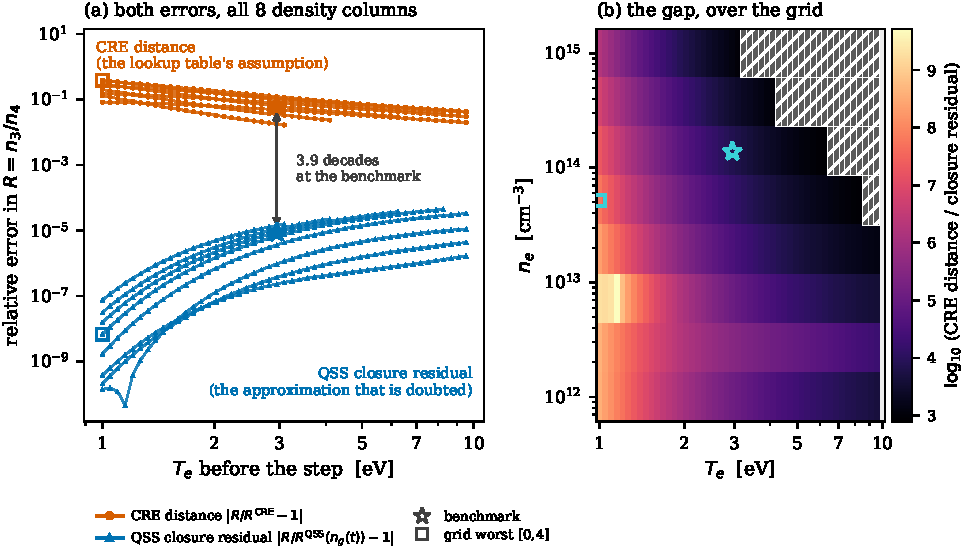
\includegraphics{figures/fig5_5_reversal.pdf}
%     \caption{\CapFigReversal}\label{fig:reversal}
%   \end{figure}

\newcommand{\CapFigReversal}{%
  \textbf{The reversal: the approximation that is doubted holds, the
  assumption that is not examined fails.}
  Two errors in the same observable, the shell ratio $R = n_3/n_4$, measured
  along the same trajectory after a $+4.81\%$ step in $T_e$ at fixed $n_e$,
  and reported as the maximum over the timescale-separated plateau window
  $30\tau_{\rm relax} < t < \tau_{\rm slow}/30$.
  The \emph{quasi-steady-state closure residual} is
  $|R(t)/R^{\rm QSS}(n_g(t)) - 1|$, where $R^{\rm QSS}$ is rebuilt at each
  instant from the excited-state block alone,
  $n_E = -L_{EE}^{-1}(L_{Eg}n_g + S_E)$, evaluated at the
  \emph{instantaneous} ground density rather than at any tabulated value.
  The \emph{CRE distance} is $|R(t)/R^{\rm CRE} - 1|$, the distance to the
  equilibrium-ionisation-balance state $n = -L^{-1}S$ that a two-parameter
  $(T_e, n_e)$ lookup table returns.
  (a) Both, for all 392 analysed cells across the 8 density
  columns. The closure residual runs from $4.6\times10^{-11}$ to $4.4\times10^{-5}$, so the
  closure everyone worries about is never worse than one part in
  $2.2\times10^{4}$ anywhere on the analysed grid: it is $8.66\times10^{-6}$ at the
  benchmark ($T_e = 2.947$~eV, $n_e = 1.4\times10^{14}$~cm$^{-3}$), one part in
  $1.2\times10^{5}$, and $6.73\times10^{-9}$ at the coldest point
  $[0,4]$, one part in $1.5\times10^{8}$.
  The CRE distance over the same cells runs from 1.66\% to 38.7\%:
  6.34\% at the benchmark and 38.7\% at the coldest point.
  The assumption nobody examines therefore fails at the tens-of-percent
  level exactly where the closure everybody examines is exact to within
  one part in $10^{5}$ or better.
  (b) The ratio of the two over the grid. The gap is 2.9 to 9.7
  decades wide, 3.9 decades at the benchmark and 7.8 decades at the
  coldest point; it is not a single number and should not be quoted as one.
  Hatched cells (54 of 392) have no timescale-separated plateau
  window, $M \leq 900$, an imposed cut rather than a measured floor.
  Trajectories are eigen-propagations of the full 43-state operator,
  sampled at 24 points across each window and checked against
  \texttt{scipy.linalg.expm} at the window midpoint of every cell, worst
  disagreement $3\times10^{-9}$.
  Values below $2$~eV are optically thin upper estimates: Lyman trapping is
  not switched on here.}

\newcommand{\CapFigTrajectory}{%
  \textbf{What the plateau looks like: the excited states keep up, the
  reservoir does not.}
  The shell ratio $R(t) = n_3/n_4$ after a step in $T_e$ at fixed $n_e$,
  on a logarithmic time axis long enough to hold both timescales.
  Three phases are visible. $R$ rises on $\tau_{\rm relax}$ as the excited
  manifold re-equilibrates against a ground state that has not yet moved; it
  sits at the partial-equilibrium value $R^{\rm PE}$; then it decays on
  $\tau_{\rm slow}$ as the ground state, and with it the ionisation balance,
  finally responds. The excited states are fast enough to track the new
  temperature within nanoseconds. The reservoir that feeds them is not.
  (a) The benchmark, $T_e = 2.947 \rightarrow 3.09$~eV at
  $n_e = 1.4\times10^{14}$~cm$^{-3}$: $R$ moves from $0.7778$ through
  $0.8201$ to $0.7711$, a plateau error of 6.36\%, with
  $\tau_{\rm relax} = 2.24\times10^{-9}$~s and $\tau_{\rm slow} = 1.85\times10^{-5}$~s
  ($M = 8243$).
  (b) The coldest grid point, $T_e = 1.00 \rightarrow 1.05$~eV at
  $n_e = 5.2\times10^{13}$~cm$^{-3}$: $1.2391$ through $1.6712$ to $1.2050$,
  38.7\%, with $\tau_{\rm relax} = 6.24\times10^{-9}$~s and
  $\tau_{\rm slow} = 0.233$~s ($M = 3.74\times10^{7}$), five orders of magnitude of
  separation between the two clocks.
  Every timescale quoted belongs to the \emph{post-step} operator, the one
  that governs the relaxation; the same grid point read from its unstepped
  operator gives a different $M$, and the two must not be interchanged.
  $R^{\rm PE}$ is computed independently by a single linear solve against
  that operator and agrees with the two-channel construction used elsewhere
  in this chapter to $2\times10^{-16}$. The plateau is flat to 0.17\%
  peak to peak in (a). Curves are eigen-propagations of the full
  43-state operator, cross-checked against \texttt{scipy.linalg.expm}
  inside the plateau window, worst disagreement $1\times10^{-7}$.}

\newcommand{\CapFigStructuralMaps}{%
  \textbf{The two structural coefficients, and the invariant they multiply
  to.}
  The plateau error obeys
  $\varepsilon = |\exp(\bar{S} G \,\mathrm{d}\ln T_e) - 1|$ exactly, which
  splits it into a part belonging to the observable and a part belonging to
  the plasma.
  (a) $|\bar{S}| = |f_3 - f_4|$, the sensitivity of the $n=3/n=4$ ratio to
  the ground-state reservoir, where $f_n$ is the ground-fed fraction of shell
  $n$.
  (b) $|G| = |\mathrm{d}\ln u / \mathrm{d}\ln T_e|$, the reservoir gain,
  measuring how far the ground population moves for a given change in
  temperature.
  (c) Their product $|\bar{S}G|$, which is the small-step limit of
  $\varepsilon/|\mathrm{d}\ln T_e|$ and is the coefficient this chapter reports
  in place of a percentage that depends on the step chosen. It is written as a
  limiting ratio and not as $\mathrm{d}\varepsilon/\mathrm{d}\ln T_e$ because
  $\varepsilon = |\mathrm{e}^z-1|$ has a corner at $z=0$, where the two-sided
  derivative does not exist. $G$ itself is a secant over the step taken, not a
  local derivative, so it carries a weak and systematic step dependence.
  All three are heating, one grid index in $T_e$
  ($\mathrm{d}\ln T_e = 0.0470$), over all 392 cells.
  Ranges quoted with their scope, because the scope changes them: over the
  338 cells drawn here that pass the plateau-window test,
  $|\bar{S}|$ runs 0.065 to 0.482 and $|G|$ runs 2.64 to 14.52, giving
  a product of 0.36 to 6.96; over all 2288 rows of the source table,
  which include cooling and larger steps, $|\bar{S}|$ runs 0.0355 to
  0.4963 while $|G|$ is unchanged at 2.64 to 14.52.
  At the benchmark $|\bar{S}| = 0.229$, $|G| = 5.74$ and the product is
  1.31.
  $G$ is what makes this reframing worth anything: across step sizes of one,
  two and four grid indices at the 736 points carrying all three, $|G|$
  varies by at most 6.74\% (median 1.0555) while $\varepsilon$ over
  the same points varies by up to a factor 8.44.
  Hatched cells (54 of 392) fail the plateau-window test
  $M > 900$; their values are drawn rather than deleted, since $\bar{S}$
  and $G$ are properties of the operator and remain defined there even where
  a plateau does not.}

\newcommand{\CapFigScope}{%
  \textbf{Two independent constraints put the same floor under the
  quantitative scope.}
  Neither boundary was chosen; both were measured, and they come from
  unrelated physics.
  \emph{Quasi-neutrality.} Imposing nuclei conservation across one grid step
  in $T_e$, the electron density must change by
  $|\Delta n_e / n_e| = |\Delta n_g| / n_{\rm ion}$, taken from the two
  CR-equilibrium solves either side of the step. This zero-dimensional model
  holds $n_e$ fixed, so wherever that requirement is large the model is
  contradicting itself. Of the 392 one-step operators on the grid,
  68 require more than $10\%$ and 36 require more than $100\%$. At
  $T_e = 1$~eV the requirement is between 10.1 and 20.0, that
  is, ten to twenty times the electron density itself. At $T_e \geq 2$~eV it
  never exceeds $0.0054$. The $10\%$ contour sits at
  $T_e = 1.41$ to 1.50~eV and is almost independent of density.
  \emph{Optical depth.} The Lyman-$\alpha$ line-centre optical depth over the
  half slab, $\tau_0 = n(1s)\,\sigma_0\,D/2$, with $\sigma_0$ evaluated at
  $T_{\rm at} = T_e$ from the Doppler width $\sqrt{2kT/m}$, giving
  $\sigma_0 = 5.474\times10^{-14}$~cm$^{2}$ at $1$~eV. The optically thin matrix used
  throughout this thesis is only defensible where $\tau_0 < 1$. That contour
  runs from $T_e = 1.13$ to 1.98~eV at the slab thickness
  $D = 5$~cm, and across the 3 thicknesses in the trapping sweep it
  spans 1.01 to 2.36~eV.
  (a) Both boundaries on the $(T_e, n_e)$ plane, over a map of the
  quasi-neutrality requirement.
  (b) Each constraint divided by its own limit, so that a value above one
  means the constraint is violated and the two can share a single axis.
  Both boundaries fall between 1.01 and 2.36~eV. Two independent
  pieces of physics, particle conservation and radiation transport, place the
  floor in the same narrow band, and $T_e \geq 2$~eV clears both everywhere
  except 2 of the 3 times eight optical-depth crossings, which sit
  at the largest slab thickness $D = 20$~cm and the two highest density
  columns. The $T_e \geq 2$~eV restriction is therefore a measured boundary,
  not a hedge.}

\newcommand{\CapFigDiagnosticChain}{%
  \textbf{Where the hidden assumption enters divertor spectroscopy.}
  The inference runs left to right. A spectrometer records the Balmer
  emission; the ratio of two line intensities, here
  $I_{{\rm H}\alpha}/I_{{\rm H}\beta}$ at $656.1$ and $486.0$~nm, reduces
  the spectrum to a single number per line of sight; that number is looked up
  in a table of the ratio computed as a function of $(T_e, n_e)$; and the
  pair that reproduces it is reported as the plasma conditions.
  The step that is rarely stated is the third. The table is built from the
  CR-equilibrium populations, so it assumes the ionisation balance has
  already settled, $n_g/n_{\rm ion} = u^{\rm CRE}(T_e, n_e)$. A plasma still
  in transit after a change in temperature does not satisfy that, and the
  inversion then returns a temperature and a density that no plasma had.
  This thesis is about the size of that error and about which of the
  approximations in the chain is actually responsible for it.
  This is a schematic. No measured or computed quantity is plotted; the two
  wavelengths are the only numbers on it, and they follow from the
  ionisation energies in the model's own state index. The drawn line heights
  are arbitrary and carry no information about the real intensity ratio.}

\newcommand{\CapFigStateSpace}{%
  \textbf{The 43-state space and the five processes the rate matrix
  contains.}
  Left: the level structure. Hydrogen is $\ell$-resolved up to
  $n = 8$, which is 36 states, and bundled into one level per $n$
  from $n = 9$ to 15, which is 7 more. Vertical spacing is
  schematic; the right-hand panel gives the true energies, and shows why,
  with 37 of the 43 states lying within 0.85~eV of the continuum,
  a to-scale ladder would be unreadable.
  Five processes appear in the matrix: electron-impact excitation and
  de-excitation between levels, radiative decay
  ($A_{2p \to 1s} = 6.27\times10^{8}$~s$^{-1}$, and 34 of the 36 resolved states
  carry a non-zero decay rate), electron-impact ionisation from every state,
  recombination, which enters as the source vector rather than as a matrix
  element and feeds every state, and proton-impact $\ell$-mixing, which is
  $\Delta n = 0$ and acts on 35 states, every resolved level with
  $n \geq 2$. Only the $n = 2$ and $n = 3$ mixing arrows are drawn; at
  $n = 4$ the sublevels are too close together for an arrow to render
  legibly.
  The dashed boxes mark the partition the analysis rests on, and $2s$ is why
  it can be drawn where it is. $2s$ has no E1 decay to the ground state, its
  radiative rate to $1s$ being exactly zero in the matrix, so on radiative
  grounds alone it would be metastable and would belong with the slow states.
  It is nonetheless fast, because proton $\ell$-mixing to $2p$ carries
  99.97\% of its total loss rate of $1.47\times10^{11}$~s$^{-1}$ at the benchmark,
  and never less than 99.92\% anywhere on the grid, rising to 99.99\%
  at the cold edge. That single channel is what leaves
  $\mathcal{S} = \{1s\}$ as the only slow state and the remaining
  42 levels in the fast manifold.
  The state list, including which levels are bundled and every ionisation
  energy, is read from the model's own state index, not written into this
  figure.}
  in the preamble, then
%   \begin{figure}[t]\centering
%     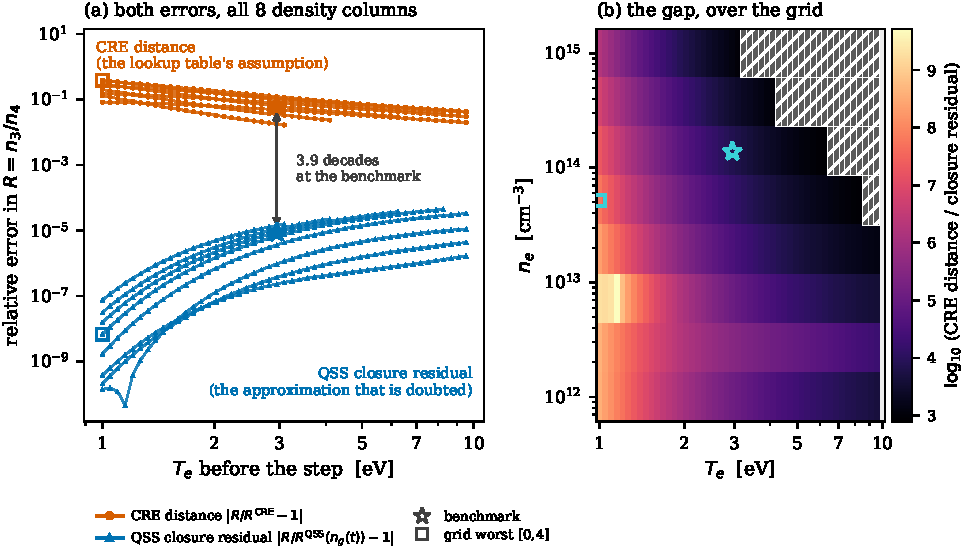
\includegraphics{figures/fig5_5_reversal.pdf}
%     \caption{\CapFigReversal}\label{fig:reversal}
%   \end{figure}

\newcommand{\CapFigReversal}{%
  \textbf{The reversal: the approximation that is doubted holds, the
  assumption that is not examined fails.}
  Two errors in the same observable, the shell ratio $R = n_3/n_4$, measured
  along the same trajectory after a $+4.81\%$ step in $T_e$ at fixed $n_e$,
  and reported as the maximum over the timescale-separated plateau window
  $30\tau_{\rm relax} < t < \tau_{\rm slow}/30$.
  The \emph{quasi-steady-state closure residual} is
  $|R(t)/R^{\rm QSS}(n_g(t)) - 1|$, where $R^{\rm QSS}$ is rebuilt at each
  instant from the excited-state block alone,
  $n_E = -L_{EE}^{-1}(L_{Eg}n_g + S_E)$, evaluated at the
  \emph{instantaneous} ground density rather than at any tabulated value.
  The \emph{CRE distance} is $|R(t)/R^{\rm CRE} - 1|$, the distance to the
  equilibrium-ionisation-balance state $n = -L^{-1}S$ that a two-parameter
  $(T_e, n_e)$ lookup table returns.
  (a) Both, for all 392 analysed cells across the 8 density
  columns. The closure residual runs from $4.6\times10^{-11}$ to $4.4\times10^{-5}$, so the
  closure everyone worries about is never worse than one part in
  $2.2\times10^{4}$ anywhere on the analysed grid: it is $8.66\times10^{-6}$ at the
  benchmark ($T_e = 2.947$~eV, $n_e = 1.4\times10^{14}$~cm$^{-3}$), one part in
  $1.2\times10^{5}$, and $6.73\times10^{-9}$ at the coldest point
  $[0,4]$, one part in $1.5\times10^{8}$.
  The CRE distance over the same cells runs from 1.66\% to 38.7\%:
  6.34\% at the benchmark and 38.7\% at the coldest point.
  The assumption nobody examines therefore fails at the tens-of-percent
  level exactly where the closure everybody examines is exact to within
  one part in $10^{5}$ or better.
  (b) The ratio of the two over the grid. The gap is 2.9 to 9.7
  decades wide, 3.9 decades at the benchmark and 7.8 decades at the
  coldest point; it is not a single number and should not be quoted as one.
  Hatched cells (54 of 392) have no timescale-separated plateau
  window, $M \leq 900$, an imposed cut rather than a measured floor.
  Trajectories are eigen-propagations of the full 43-state operator,
  sampled at 24 points across each window and checked against
  \texttt{scipy.linalg.expm} at the window midpoint of every cell, worst
  disagreement $3\times10^{-9}$.
  Values below $2$~eV are optically thin upper estimates: Lyman trapping is
  not switched on here.}

\newcommand{\CapFigTrajectory}{%
  \textbf{What the plateau looks like: the excited states keep up, the
  reservoir does not.}
  The shell ratio $R(t) = n_3/n_4$ after a step in $T_e$ at fixed $n_e$,
  on a logarithmic time axis long enough to hold both timescales.
  Three phases are visible. $R$ rises on $\tau_{\rm relax}$ as the excited
  manifold re-equilibrates against a ground state that has not yet moved; it
  sits at the partial-equilibrium value $R^{\rm PE}$; then it decays on
  $\tau_{\rm slow}$ as the ground state, and with it the ionisation balance,
  finally responds. The excited states are fast enough to track the new
  temperature within nanoseconds. The reservoir that feeds them is not.
  (a) The benchmark, $T_e = 2.947 \rightarrow 3.09$~eV at
  $n_e = 1.4\times10^{14}$~cm$^{-3}$: $R$ moves from $0.7778$ through
  $0.8201$ to $0.7711$, a plateau error of 6.36\%, with
  $\tau_{\rm relax} = 2.24\times10^{-9}$~s and $\tau_{\rm slow} = 1.85\times10^{-5}$~s
  ($M = 8243$).
  (b) The coldest grid point, $T_e = 1.00 \rightarrow 1.05$~eV at
  $n_e = 5.2\times10^{13}$~cm$^{-3}$: $1.2391$ through $1.6712$ to $1.2050$,
  38.7\%, with $\tau_{\rm relax} = 6.24\times10^{-9}$~s and
  $\tau_{\rm slow} = 0.233$~s ($M = 3.74\times10^{7}$), five orders of magnitude of
  separation between the two clocks.
  Every timescale quoted belongs to the \emph{post-step} operator, the one
  that governs the relaxation; the same grid point read from its unstepped
  operator gives a different $M$, and the two must not be interchanged.
  $R^{\rm PE}$ is computed independently by a single linear solve against
  that operator and agrees with the two-channel construction used elsewhere
  in this chapter to $2\times10^{-16}$. The plateau is flat to 0.17\%
  peak to peak in (a). Curves are eigen-propagations of the full
  43-state operator, cross-checked against \texttt{scipy.linalg.expm}
  inside the plateau window, worst disagreement $1\times10^{-7}$.}

\newcommand{\CapFigStructuralMaps}{%
  \textbf{The two structural coefficients, and the invariant they multiply
  to.}
  The plateau error obeys
  $\varepsilon = |\exp(\bar{S} G \,\mathrm{d}\ln T_e) - 1|$ exactly, which
  splits it into a part belonging to the observable and a part belonging to
  the plasma.
  (a) $|\bar{S}| = |f_3 - f_4|$, the sensitivity of the $n=3/n=4$ ratio to
  the ground-state reservoir, where $f_n$ is the ground-fed fraction of shell
  $n$.
  (b) $|G| = |\mathrm{d}\ln u / \mathrm{d}\ln T_e|$, the reservoir gain,
  measuring how far the ground population moves for a given change in
  temperature.
  (c) Their product $|\bar{S}G|$, which is the small-step limit of
  $\varepsilon/|\mathrm{d}\ln T_e|$ and is the coefficient this chapter reports
  in place of a percentage that depends on the step chosen. It is written as a
  limiting ratio and not as $\mathrm{d}\varepsilon/\mathrm{d}\ln T_e$ because
  $\varepsilon = |\mathrm{e}^z-1|$ has a corner at $z=0$, where the two-sided
  derivative does not exist. $G$ itself is a secant over the step taken, not a
  local derivative, so it carries a weak and systematic step dependence.
  All three are heating, one grid index in $T_e$
  ($\mathrm{d}\ln T_e = 0.0470$), over all 392 cells.
  Ranges quoted with their scope, because the scope changes them: over the
  338 cells drawn here that pass the plateau-window test,
  $|\bar{S}|$ runs 0.065 to 0.482 and $|G|$ runs 2.64 to 14.52, giving
  a product of 0.36 to 6.96; over all 2288 rows of the source table,
  which include cooling and larger steps, $|\bar{S}|$ runs 0.0355 to
  0.4963 while $|G|$ is unchanged at 2.64 to 14.52.
  At the benchmark $|\bar{S}| = 0.229$, $|G| = 5.74$ and the product is
  1.31.
  $G$ is what makes this reframing worth anything: across step sizes of one,
  two and four grid indices at the 736 points carrying all three, $|G|$
  varies by at most 6.74\% (median 1.0555) while $\varepsilon$ over
  the same points varies by up to a factor 8.44.
  Hatched cells (54 of 392) fail the plateau-window test
  $M > 900$; their values are drawn rather than deleted, since $\bar{S}$
  and $G$ are properties of the operator and remain defined there even where
  a plateau does not.}

\newcommand{\CapFigScope}{%
  \textbf{Two independent constraints put the same floor under the
  quantitative scope.}
  Neither boundary was chosen; both were measured, and they come from
  unrelated physics.
  \emph{Quasi-neutrality.} Imposing nuclei conservation across one grid step
  in $T_e$, the electron density must change by
  $|\Delta n_e / n_e| = |\Delta n_g| / n_{\rm ion}$, taken from the two
  CR-equilibrium solves either side of the step. This zero-dimensional model
  holds $n_e$ fixed, so wherever that requirement is large the model is
  contradicting itself. Of the 392 one-step operators on the grid,
  68 require more than $10\%$ and 36 require more than $100\%$. At
  $T_e = 1$~eV the requirement is between 10.1 and 20.0, that
  is, ten to twenty times the electron density itself. At $T_e \geq 2$~eV it
  never exceeds $0.0054$. The $10\%$ contour sits at
  $T_e = 1.41$ to 1.50~eV and is almost independent of density.
  \emph{Optical depth.} The Lyman-$\alpha$ line-centre optical depth over the
  half slab, $\tau_0 = n(1s)\,\sigma_0\,D/2$, with $\sigma_0$ evaluated at
  $T_{\rm at} = T_e$ from the Doppler width $\sqrt{2kT/m}$, giving
  $\sigma_0 = 5.474\times10^{-14}$~cm$^{2}$ at $1$~eV. The optically thin matrix used
  throughout this thesis is only defensible where $\tau_0 < 1$. That contour
  runs from $T_e = 1.13$ to 1.98~eV at the slab thickness
  $D = 5$~cm, and across the 3 thicknesses in the trapping sweep it
  spans 1.01 to 2.36~eV.
  (a) Both boundaries on the $(T_e, n_e)$ plane, over a map of the
  quasi-neutrality requirement.
  (b) Each constraint divided by its own limit, so that a value above one
  means the constraint is violated and the two can share a single axis.
  Both boundaries fall between 1.01 and 2.36~eV. Two independent
  pieces of physics, particle conservation and radiation transport, place the
  floor in the same narrow band, and $T_e \geq 2$~eV clears both everywhere
  except 2 of the 3 times eight optical-depth crossings, which sit
  at the largest slab thickness $D = 20$~cm and the two highest density
  columns. The $T_e \geq 2$~eV restriction is therefore a measured boundary,
  not a hedge.}

\newcommand{\CapFigDiagnosticChain}{%
  \textbf{Where the hidden assumption enters divertor spectroscopy.}
  The inference runs left to right. A spectrometer records the Balmer
  emission; the ratio of two line intensities, here
  $I_{{\rm H}\alpha}/I_{{\rm H}\beta}$ at $656.1$ and $486.0$~nm, reduces
  the spectrum to a single number per line of sight; that number is looked up
  in a table of the ratio computed as a function of $(T_e, n_e)$; and the
  pair that reproduces it is reported as the plasma conditions.
  The step that is rarely stated is the third. The table is built from the
  CR-equilibrium populations, so it assumes the ionisation balance has
  already settled, $n_g/n_{\rm ion} = u^{\rm CRE}(T_e, n_e)$. A plasma still
  in transit after a change in temperature does not satisfy that, and the
  inversion then returns a temperature and a density that no plasma had.
  This thesis is about the size of that error and about which of the
  approximations in the chain is actually responsible for it.
  This is a schematic. No measured or computed quantity is plotted; the two
  wavelengths are the only numbers on it, and they follow from the
  ionisation energies in the model's own state index. The drawn line heights
  are arbitrary and carry no information about the real intensity ratio.}

\newcommand{\CapFigStateSpace}{%
  \textbf{The 43-state space and the five processes the rate matrix
  contains.}
  Left: the level structure. Hydrogen is $\ell$-resolved up to
  $n = 8$, which is 36 states, and bundled into one level per $n$
  from $n = 9$ to 15, which is 7 more. Vertical spacing is
  schematic; the right-hand panel gives the true energies, and shows why,
  with 37 of the 43 states lying within 0.85~eV of the continuum,
  a to-scale ladder would be unreadable.
  Five processes appear in the matrix: electron-impact excitation and
  de-excitation between levels, radiative decay
  ($A_{2p \to 1s} = 6.27\times10^{8}$~s$^{-1}$, and 34 of the 36 resolved states
  carry a non-zero decay rate), electron-impact ionisation from every state,
  recombination, which enters as the source vector rather than as a matrix
  element and feeds every state, and proton-impact $\ell$-mixing, which is
  $\Delta n = 0$ and acts on 35 states, every resolved level with
  $n \geq 2$. Only the $n = 2$ and $n = 3$ mixing arrows are drawn; at
  $n = 4$ the sublevels are too close together for an arrow to render
  legibly.
  The dashed boxes mark the partition the analysis rests on, and $2s$ is why
  it can be drawn where it is. $2s$ has no E1 decay to the ground state, its
  radiative rate to $1s$ being exactly zero in the matrix, so on radiative
  grounds alone it would be metastable and would belong with the slow states.
  It is nonetheless fast, because proton $\ell$-mixing to $2p$ carries
  99.97\% of its total loss rate of $1.47\times10^{11}$~s$^{-1}$ at the benchmark,
  and never less than 99.92\% anywhere on the grid, rising to 99.99\%
  at the cold edge. That single channel is what leaves
  $\mathcal{S} = \{1s\}$ as the only slow state and the remaining
  42 levels in the fast manifold.
  The state list, including which levels are bundled and every ionisation
  energy, is read from the model's own state index, not written into this
  figure.}
  in the preamble, then
%   \begin{figure}[t]\centering
%     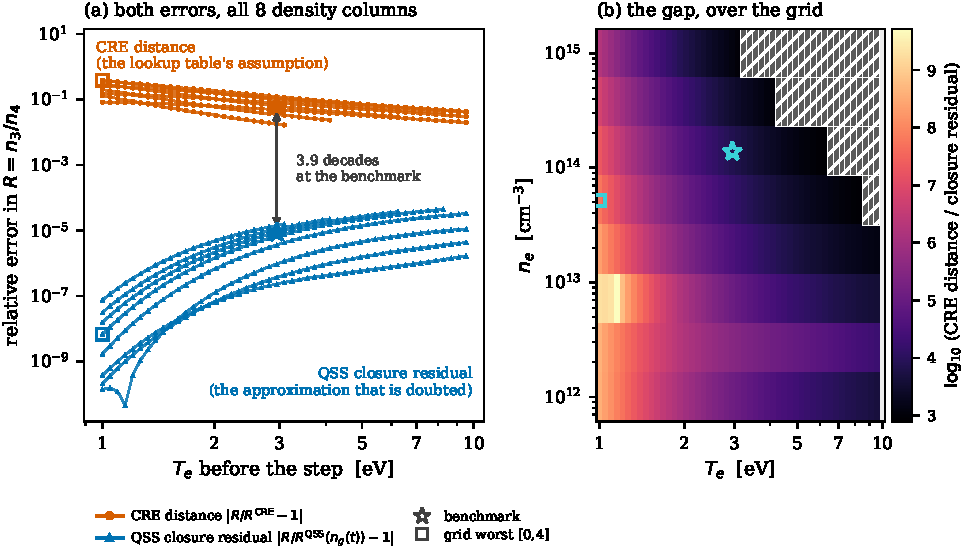
\includegraphics{figures/fig5_5_reversal.pdf}
%     \caption{\CapFigReversal}\label{fig:reversal}
%   \end{figure}

\newcommand{\CapFigReversal}{%
  \textbf{The reversal: the approximation that is doubted holds, the
  assumption that is not examined fails.}
  Two errors in the same observable, the shell ratio $R = n_3/n_4$, measured
  along the same trajectory after a $+4.81\%$ step in $T_e$ at fixed $n_e$,
  and reported as the maximum over the timescale-separated plateau window
  $30\tau_{\rm relax} < t < \tau_{\rm slow}/30$.
  The \emph{quasi-steady-state closure residual} is
  $|R(t)/R^{\rm QSS}(n_g(t)) - 1|$, where $R^{\rm QSS}$ is rebuilt at each
  instant from the excited-state block alone,
  $n_E = -L_{EE}^{-1}(L_{Eg}n_g + S_E)$, evaluated at the
  \emph{instantaneous} ground density rather than at any tabulated value.
  The \emph{CRE distance} is $|R(t)/R^{\rm CRE} - 1|$, the distance to the
  equilibrium-ionisation-balance state $n = -L^{-1}S$ that a two-parameter
  $(T_e, n_e)$ lookup table returns.
  (a) Both, for all 392 analysed cells across the 8 density
  columns. The closure residual runs from $4.6\times10^{-11}$ to $4.4\times10^{-5}$, so the
  closure everyone worries about is never worse than one part in
  $2.2\times10^{4}$ anywhere on the analysed grid: it is $8.66\times10^{-6}$ at the
  benchmark ($T_e = 2.947$~eV, $n_e = 1.4\times10^{14}$~cm$^{-3}$), one part in
  $1.2\times10^{5}$, and $6.73\times10^{-9}$ at the coldest point
  $[0,4]$, one part in $1.5\times10^{8}$.
  The CRE distance over the same cells runs from 1.66\% to 38.7\%:
  6.34\% at the benchmark and 38.7\% at the coldest point.
  The assumption nobody examines therefore fails at the tens-of-percent
  level exactly where the closure everybody examines is exact to within
  one part in $10^{5}$ or better.
  (b) The ratio of the two over the grid. The gap is 2.9 to 9.7
  decades wide, 3.9 decades at the benchmark and 7.8 decades at the
  coldest point; it is not a single number and should not be quoted as one.
  Hatched cells (54 of 392) have no timescale-separated plateau
  window, $M \leq 900$, an imposed cut rather than a measured floor.
  Trajectories are eigen-propagations of the full 43-state operator,
  sampled at 24 points across each window and checked against
  \texttt{scipy.linalg.expm} at the window midpoint of every cell, worst
  disagreement $3\times10^{-9}$.
  Values below $2$~eV are optically thin upper estimates: Lyman trapping is
  not switched on here.}

\newcommand{\CapFigTrajectory}{%
  \textbf{What the plateau looks like: the excited states keep up, the
  reservoir does not.}
  The shell ratio $R(t) = n_3/n_4$ after a step in $T_e$ at fixed $n_e$,
  on a logarithmic time axis long enough to hold both timescales.
  Three phases are visible. $R$ rises on $\tau_{\rm relax}$ as the excited
  manifold re-equilibrates against a ground state that has not yet moved; it
  sits at the partial-equilibrium value $R^{\rm PE}$; then it decays on
  $\tau_{\rm slow}$ as the ground state, and with it the ionisation balance,
  finally responds. The excited states are fast enough to track the new
  temperature within nanoseconds. The reservoir that feeds them is not.
  (a) The benchmark, $T_e = 2.947 \rightarrow 3.09$~eV at
  $n_e = 1.4\times10^{14}$~cm$^{-3}$: $R$ moves from $0.7778$ through
  $0.8201$ to $0.7711$, a plateau error of 6.36\%, with
  $\tau_{\rm relax} = 2.24\times10^{-9}$~s and $\tau_{\rm slow} = 1.85\times10^{-5}$~s
  ($M = 8243$).
  (b) The coldest grid point, $T_e = 1.00 \rightarrow 1.05$~eV at
  $n_e = 5.2\times10^{13}$~cm$^{-3}$: $1.2391$ through $1.6712$ to $1.2050$,
  38.7\%, with $\tau_{\rm relax} = 6.24\times10^{-9}$~s and
  $\tau_{\rm slow} = 0.233$~s ($M = 3.74\times10^{7}$), five orders of magnitude of
  separation between the two clocks.
  Every timescale quoted belongs to the \emph{post-step} operator, the one
  that governs the relaxation; the same grid point read from its unstepped
  operator gives a different $M$, and the two must not be interchanged.
  $R^{\rm PE}$ is computed independently by a single linear solve against
  that operator and agrees with the two-channel construction used elsewhere
  in this chapter to $2\times10^{-16}$. The plateau is flat to 0.17\%
  peak to peak in (a). Curves are eigen-propagations of the full
  43-state operator, cross-checked against \texttt{scipy.linalg.expm}
  inside the plateau window, worst disagreement $1\times10^{-7}$.}

\newcommand{\CapFigStructuralMaps}{%
  \textbf{The two structural coefficients, and the invariant they multiply
  to.}
  The plateau error obeys
  $\varepsilon = |\exp(\bar{S} G \,\mathrm{d}\ln T_e) - 1|$ exactly, which
  splits it into a part belonging to the observable and a part belonging to
  the plasma.
  (a) $|\bar{S}| = |f_3 - f_4|$, the sensitivity of the $n=3/n=4$ ratio to
  the ground-state reservoir, where $f_n$ is the ground-fed fraction of shell
  $n$.
  (b) $|G| = |\mathrm{d}\ln u / \mathrm{d}\ln T_e|$, the reservoir gain,
  measuring how far the ground population moves for a given change in
  temperature.
  (c) Their product $|\bar{S}G|$, which is the small-step limit of
  $\varepsilon/|\mathrm{d}\ln T_e|$ and is the coefficient this chapter reports
  in place of a percentage that depends on the step chosen. It is written as a
  limiting ratio and not as $\mathrm{d}\varepsilon/\mathrm{d}\ln T_e$ because
  $\varepsilon = |\mathrm{e}^z-1|$ has a corner at $z=0$, where the two-sided
  derivative does not exist. $G$ itself is a secant over the step taken, not a
  local derivative, so it carries a weak and systematic step dependence.
  All three are heating, one grid index in $T_e$
  ($\mathrm{d}\ln T_e = 0.0470$), over all 392 cells.
  Ranges quoted with their scope, because the scope changes them: over the
  338 cells drawn here that pass the plateau-window test,
  $|\bar{S}|$ runs 0.065 to 0.482 and $|G|$ runs 2.64 to 14.52, giving
  a product of 0.36 to 6.96; over all 2288 rows of the source table,
  which include cooling and larger steps, $|\bar{S}|$ runs 0.0355 to
  0.4963 while $|G|$ is unchanged at 2.64 to 14.52.
  At the benchmark $|\bar{S}| = 0.229$, $|G| = 5.74$ and the product is
  1.31.
  $G$ is what makes this reframing worth anything: across step sizes of one,
  two and four grid indices at the 736 points carrying all three, $|G|$
  varies by at most 6.74\% (median 1.0555) while $\varepsilon$ over
  the same points varies by up to a factor 8.44.
  Hatched cells (54 of 392) fail the plateau-window test
  $M > 900$; their values are drawn rather than deleted, since $\bar{S}$
  and $G$ are properties of the operator and remain defined there even where
  a plateau does not.}

\newcommand{\CapFigScope}{%
  \textbf{Two independent constraints put the same floor under the
  quantitative scope.}
  Neither boundary was chosen; both were measured, and they come from
  unrelated physics.
  \emph{Quasi-neutrality.} Imposing nuclei conservation across one grid step
  in $T_e$, the electron density must change by
  $|\Delta n_e / n_e| = |\Delta n_g| / n_{\rm ion}$, taken from the two
  CR-equilibrium solves either side of the step. This zero-dimensional model
  holds $n_e$ fixed, so wherever that requirement is large the model is
  contradicting itself. Of the 392 one-step operators on the grid,
  68 require more than $10\%$ and 36 require more than $100\%$. At
  $T_e = 1$~eV the requirement is between 10.1 and 20.0, that
  is, ten to twenty times the electron density itself. At $T_e \geq 2$~eV it
  never exceeds $0.0054$. The $10\%$ contour sits at
  $T_e = 1.41$ to 1.50~eV and is almost independent of density.
  \emph{Optical depth.} The Lyman-$\alpha$ line-centre optical depth over the
  half slab, $\tau_0 = n(1s)\,\sigma_0\,D/2$, with $\sigma_0$ evaluated at
  $T_{\rm at} = T_e$ from the Doppler width $\sqrt{2kT/m}$, giving
  $\sigma_0 = 5.474\times10^{-14}$~cm$^{2}$ at $1$~eV. The optically thin matrix used
  throughout this thesis is only defensible where $\tau_0 < 1$. That contour
  runs from $T_e = 1.13$ to 1.98~eV at the slab thickness
  $D = 5$~cm, and across the 3 thicknesses in the trapping sweep it
  spans 1.01 to 2.36~eV.
  (a) Both boundaries on the $(T_e, n_e)$ plane, over a map of the
  quasi-neutrality requirement.
  (b) Each constraint divided by its own limit, so that a value above one
  means the constraint is violated and the two can share a single axis.
  Both boundaries fall between 1.01 and 2.36~eV. Two independent
  pieces of physics, particle conservation and radiation transport, place the
  floor in the same narrow band, and $T_e \geq 2$~eV clears both everywhere
  except 2 of the 3 times eight optical-depth crossings, which sit
  at the largest slab thickness $D = 20$~cm and the two highest density
  columns. The $T_e \geq 2$~eV restriction is therefore a measured boundary,
  not a hedge.}

\newcommand{\CapFigDiagnosticChain}{%
  \textbf{Where the hidden assumption enters divertor spectroscopy.}
  The inference runs left to right. A spectrometer records the Balmer
  emission; the ratio of two line intensities, here
  $I_{{\rm H}\alpha}/I_{{\rm H}\beta}$ at $656.1$ and $486.0$~nm, reduces
  the spectrum to a single number per line of sight; that number is looked up
  in a table of the ratio computed as a function of $(T_e, n_e)$; and the
  pair that reproduces it is reported as the plasma conditions.
  The step that is rarely stated is the third. The table is built from the
  CR-equilibrium populations, so it assumes the ionisation balance has
  already settled, $n_g/n_{\rm ion} = u^{\rm CRE}(T_e, n_e)$. A plasma still
  in transit after a change in temperature does not satisfy that, and the
  inversion then returns a temperature and a density that no plasma had.
  This thesis is about the size of that error and about which of the
  approximations in the chain is actually responsible for it.
  This is a schematic. No measured or computed quantity is plotted; the two
  wavelengths are the only numbers on it, and they follow from the
  ionisation energies in the model's own state index. The drawn line heights
  are arbitrary and carry no information about the real intensity ratio.}

\newcommand{\CapFigStateSpace}{%
  \textbf{The 43-state space and the five processes the rate matrix
  contains.}
  Left: the level structure. Hydrogen is $\ell$-resolved up to
  $n = 8$, which is 36 states, and bundled into one level per $n$
  from $n = 9$ to 15, which is 7 more. Vertical spacing is
  schematic; the right-hand panel gives the true energies, and shows why,
  with 37 of the 43 states lying within 0.85~eV of the continuum,
  a to-scale ladder would be unreadable.
  Five processes appear in the matrix: electron-impact excitation and
  de-excitation between levels, radiative decay
  ($A_{2p \to 1s} = 6.27\times10^{8}$~s$^{-1}$, and 34 of the 36 resolved states
  carry a non-zero decay rate), electron-impact ionisation from every state,
  recombination, which enters as the source vector rather than as a matrix
  element and feeds every state, and proton-impact $\ell$-mixing, which is
  $\Delta n = 0$ and acts on 35 states, every resolved level with
  $n \geq 2$. Only the $n = 2$ and $n = 3$ mixing arrows are drawn; at
  $n = 4$ the sublevels are too close together for an arrow to render
  legibly.
  The dashed boxes mark the partition the analysis rests on, and $2s$ is why
  it can be drawn where it is. $2s$ has no E1 decay to the ground state, its
  radiative rate to $1s$ being exactly zero in the matrix, so on radiative
  grounds alone it would be metastable and would belong with the slow states.
  It is nonetheless fast, because proton $\ell$-mixing to $2p$ carries
  99.97\% of its total loss rate of $1.47\times10^{11}$~s$^{-1}$ at the benchmark,
  and never less than 99.92\% anywhere on the grid, rising to 99.99\%
  at the cold edge. That single channel is what leaves
  $\mathcal{S} = \{1s\}$ as the only slow state and the remaining
  42 levels in the fast manifold.
  The state list, including which levels are bundled and every ionisation
  energy, is read from the model's own state index, not written into this
  figure.}
